\section{Latency Overhead}

Network latency is the delay from the input of the system to the desired output of the system. For our case, latency is the time for the data point to propagate from one node to the next node. Latency greatly affects how usable the system is. This also brings in the question whether the system can handle a large amount of sending and receiving messages while having minimum latency so that the data is available much more quickly for querying. 
This is significant for the user to know the limitation of the system and the latency overhead the system encounter so that they could be anticipated before deploying it in their own setup.

We performed several experiments with different provenance configurations and experiments completely without provenance while keeping the sensor parameter constant to determine how big the impact of the provenance system is on the architecture. We also wanted to determine which setting has more impact on the latency and which has less to give a recommendation on a possible best setup. We did the benchmarks for different topologies that stand for usual patterns in real-world topologies. For each topology we will describe our assumptions and then evaluate the results of that.

\subsection{Test Setup and Configuration} \label{testsetup}
To run the benchmarks we used Amazon as the Cloud provider, which is an industry standard for hosting scalable services. We use Amazon Elastic Container Service which is a highly scalable, high-performance container orchestration service that supports Docker containers and allows you to easily run and scale containerized applications on AWS. In order to minimize the effect of AWS CPU and I/O variability, we performed each test three times on three different periods of different days.  New instances of t2.large\footnote{Hardware specification : \texttt{https://aws.amazon.com/ec2/instance-types/t2/} } EC2 instances, using the already configured auto-scaling group  was used to further reduce the impact of the lame instance and noisy neighbor on the benchmark results. 


\paragraph*{Executing the benchmark}
To run the benchmark on each topology, we wrote a script\footnote{Link:\url{https://github.com/Krymnos/idp-benchmark/blob/benchmark-latency/benchmark_template.sh} } which takes two parameters: the topology to run in the docker-compose file and the internet protocol address of the EC2 instance.

\begin{figure}[H]
	\center
	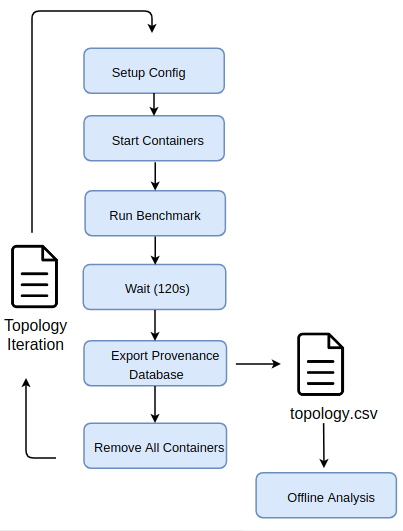
\includegraphics[width=0.5\textwidth]{figures/benchmark_latency.png}
	\caption{Benchmark Procedure}
	\label{fig:benchmark_latency}
\end{figure}

The benchmark runs the above steps for each combination of topologies described in the docker-compose file. The container is started by the docker-compose. After the "Run Benchmark" step the script waits for 120 seconds until it starts to "Export Database(Provenance Database)". There is no need to stop and start the sensor as we are measuring the time for each particular data point propagated through the pipeline. The retrieved benchmarks results are stored in the CSV file for further evaluation. After "Exporting the Database" all containers are stopped and removed to guarantee that no run is influenced by a preceding run by already "used" containers.

The field of measurement for the benchmark are:
\begin{itemize}
	\item TOPOLOGY - the topology file that was used for the run
	\item PROV\_METRICS - provenance metrics that was inserted to the config
	\item BUFFER\_CAPACITY - provenance buffer config (kept constant at 10)
	\item BENCHMARK\_RUNTIME - runtime in seconds for the benchmark (120 seconds for each run)
	\item TIME-TAKEN-FOR-ONE-HOP - Time taken by the data point to propagate from one node to the next one.
	\item TIME-TAKEN-TO-TRAVERSE-THE-PIPELINE - Time taken for the data point to propagate from the starting node to the end node.
	\item MEAN LATENCY FOR HOP - (TIME-TAKEN-FOR-ONE-HOP/ TOTAL DATAPOINT )
	\item MEAN LATENCY FOR PIPELINE - (TIME-TAKEN-TO-TRAVERSE-THE-PIPELINE/ TOTAL DATAPOINT )
\end{itemize}

For every topology we run the benchmark procedure \ref{fig:benchmark_latency} while changing only the number of context parameters at a time as shown below:

\begin{itemize}
	\item FULL CONTEXT - Provenance meterics used in the setting are :
	meterid,metricid,loc,line,class,app,ctime,stime,rtime
	\item SIX CONTEXT - Provenance meterics used in the setting are :
	meterid,metricid,app,ctime,stime,rtime
	\item FOUR CONTEXT - Provenance meterics used in the setting are :
	metricid,ctime,stime,rtime
\end{itemize}


\subsection{Two-Node Topology}
This is the base case for the latency overhead benchmark as we need to know the latency overhead of the system when we are running with bare minimal requirements to conduct the benchmark. This will provide us the threshold so that we could differentiate when running with different configuration of the system and topologies. This topology consists of one sensor and two pipeline nodes (Gateway, Endpoint) which produce provenance data. 

\begin{figure}[H]
	\center
	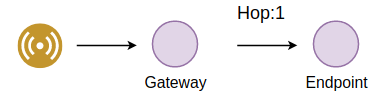
\includegraphics[width=0.5\textwidth]{figures/latencytopo_two.png}
	\caption{Two-Node Topology}
	\label{fig:two_topo}
\end{figure}

We run the topology with full context, six context parameters, four and with no provenance. We evaluated the results by plotting the mean node latency for a collection of data points
to travel from Gateway to the Endpoint labeled as Hop:1.

\begin{figure}[H]
	\center
	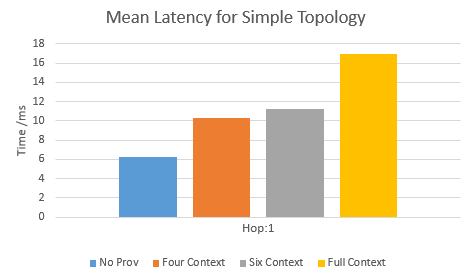
\includegraphics[width=\textwidth]{figures/simpletopology_latency.png}
	\caption{Mean Latency for collected Data-points (Two Node Topology)}
	\label{fig:twotopology_latency}
\end{figure}

From the diagram \ref{fig:twotopology_latency}, its is clearly shown that the message propagating without provenance information has the smallest latency. Furthermore, we can see a clear difference in the latency when using full context compare to using six or four context parameters for running the provenance system. Mean latency for Two Node Topology\ref{fig:two_topo} using six contexts or four context does not depict a large difference. Possible reasons for this could be the sizes of messages, as well as the amount of computations needed to collect and package the information.


\subsection*{Triangle Topology}The idea behind using this topology for the next benchmark is to check if there is any fluctuation or changes in the reading when adding another gateway to send data point to the endpoint. This will help us to check how the provenance system performs in case of adding nodes vertically to the architecture. The Triangle topology consists of two sensor nodes which send the measurements to two different gateways. These gateways (Gateway A, B) push the data to a common Endpoint.

\begin{figure}[H]
	\center
	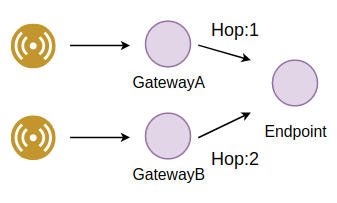
\includegraphics[width=0.5\textwidth]{figures/latencytopo_triangle.png}
	\caption{Triangle-Node Topology}
	\label{fig:triangle_topo}
\end{figure}

We run the topology with full context, six context,four context and with no provenance. We evaluated the results by plotting the mean node latency for a collected of data points
to travel from Gateway (A,B) to the Endpoint labeled as Hop:1  and Hop:2.
\begin{figure}[H]
	\center
	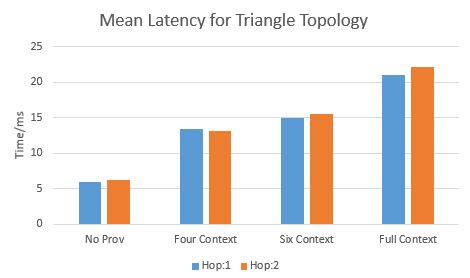
\includegraphics[width=\textwidth]{figures/triangletopology_latency.PNG}
	\caption{Mean Latency for collected Data-points  (Triangle Node Topology)}
	\label{fig:triangletopology_latency}
\end{figure}


From the diagram \ref{fig:triangletopology_latency}, the mean latency per both hops are similar. There is not much difference in mean time to travel from the Gateways(A, B) to Endpoint but there is a clear difference to the mean latency compare to the figure \ref{fig:twotopology_latency} that the mean latency increase for the all four experiment. The reason behind this might be that the Endpoint is receiving messages from two nodes instead of one node thus there is a visible difference in the measurement which is around ~8 percent average increase in mean latency. There is visible performance degradation when a single node is receiving messages from two nodes as seen from the benchmark results.

\subsection{Line Topology}
The idea behind using this topology for the next benchmark is to check if there is any visible impact on latency when adding another gateway between the endpoint and the first gateway. This will check how the provenance system performs in case of increasing node horizontally to the architecture.The Line topology consists of one sensor node which send the measurements to next gatewayA, which propagates the data to gatewayB, which then push the data to Endpoint. 

\begin{figure}[H]
	\center
	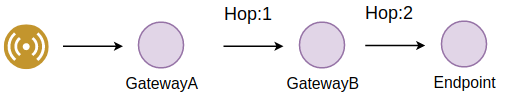
\includegraphics[width=0.5\textwidth]{figures/latencytopo_line.png}
	\caption{Line-Node Topology}
	\label{fig:line_topo}
\end{figure}

We run the topology with full context, six context,four context and with no provenance. We evaluated the results by plotting the mean node latency for a collected of data points
to travel from GatewayA to the GatewayB labeled as Hop:1  and from GatewayB to Endpoint labeled as Hop:2.

The benchmark will also give a view how the latency of the node changes when it is receiving and sending messages concurrently to the next node and the provenance database.

\begin{figure}[H]
	\center
	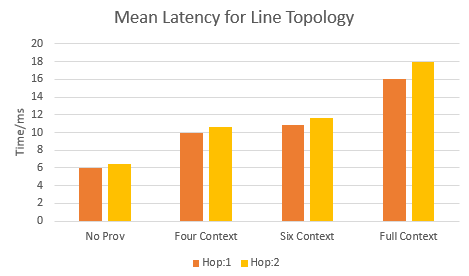
\includegraphics[width=\textwidth]{figures/LineTopology_latency.PNG}
	\caption{Mean Latency for collected Data-points   (Line Node Topology)}
	\label{fig:linetopology_latency}
\end{figure}


\begin{figure}[H]
	\center
	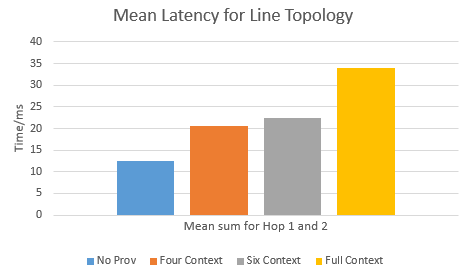
\includegraphics[width=\textwidth]{figures/LineTopology_latency_sum.PNG}
	\caption{Summation of Mean Latency for collected Data-points   (Line Node Topology)}
	\label{fig:linetopology_sum_latency}
\end{figure}

The diagram \ref{fig:linetopology_latency}  shows a visible increase in mean latency for both the hops compared to the diagram in \ref{fig:twotopology_latency} where the node was only responsible for receiving the data point. Also seen from the figure \ref{fig:linetopology_latency} the mean latency is always greater than for all the experiment for Hop:2. This is due to the GatewayB\ref{fig:line_topo} is responsible for receiving and sending the message across the pipeline explains the increased latency for both cases discussed.

Figure \ref{fig:linetopology_sum_latency} shows that due to small increase in latency on the gatewayB there is a visible difference when changing the contexts parameters from six to full especially in the case when the node is responsible of sending and receiving data-points along the node.


\subsection{Fork Node Topology}
The aim for this benchmark is to see the combined effect of increasing the nodes horizontally and vertically in the architecture and evaluate the latency overhead for the pipeline. The Fork-Node topology consists of two sensor nodes which send the measurements to two different gateways. These gateways (Gateway A,B) push the data to a common GatewayC. This Gateway C sends the data further to another endpoint node.

\begin{figure}[H]
	\center
	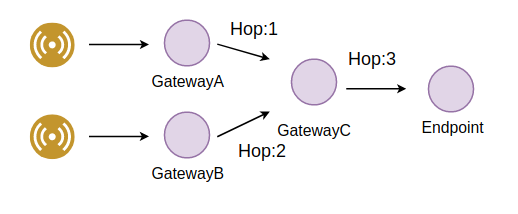
\includegraphics[width=0.5\textwidth]{figures/latencytopo_fork.png}
	\caption{Fork Node Topology}
	\label{fig:fork_topo}
\end{figure}

We ran the topology with full context, six context,four context and with no provenance. We evaluated the results by plotting the mean node latency for a collected of data points
to travel from Gateway (A,B) to the Gateway C labeled as Hop:1  and Hop:2. And Also from Gateway C to Endpoint labeled as Hop:3

\paragraph*{Assumption:}
The pipeline design is in such as way that the gatewayC receives data from two nodes and is sending the data to the endpoint. In this particular case, the majority difference of latency will be caused by this node due to congestion in network traffic.

\begin{figure}[H]
	\center
	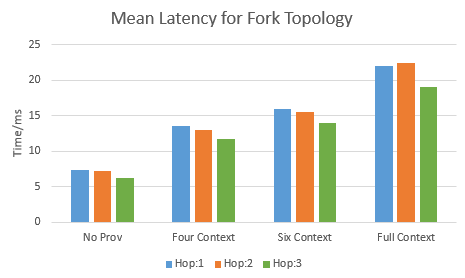
\includegraphics[width=\textwidth]{figures/ForkTopology_latency.PNG}
	\caption{Mean Latency per Data point  (Two Node Topology)}
	\label{fig:forktopo_latency}
\end{figure}

The diagram \ref{fig:forktopo_latency} shows that the mean latency for Hop:1 and Hop:2 are similar to the triangle case \ref{fig:triangle_topo} which a a bit higher then the base case \ref{fig:simple_topo}. There is a decrease in the mean latency for Hop:3 as the endpoint is only receiving data from the gatewayC which explains the node have the most number of connection with the provenance database and the next node will be the bottleneck in the system. 

\paragraph*{Conclusion}
After looking at the execution of Benchmarks for different settings, it is clear that using less context parameters with the provenance system result in less latency overhead. 
The end user should keep these results in mind when considering which parameters are relevant to track.
However, for the use case of the grid administrators where humans are reacting to failure notifications, it seems fair to say that using all 10 context parameters is feasible, since one or two seconds faster response time will not make much of a difference.
It can also be seen from the benchmarks results that the mean node latency for each hop remains consistent with no drastic changes when increasing the hops in the pipeline design, suggesting a good scalability of the system, at least for a small scale deployment such as we had the resources to test.


\paragraph*{Changing the Buffer Capacity}
After analyzing the effect of changing context parameter setting of the provenance system we need to see the effect of buffer capacity on the system in term of latency so that we know the capacity at which the system ingest data with minimal overhead. In this we want to know that if the data ingestion rate of the provenance system effect the node latency or not.
Everything was kept same as in the test setup \ref{testsetup} beside the Buffer Capacity : (10,50,100) running only on Fork Node Topology\ref{fig:fork_topo}.

\begin{figure}[H]
	\center
	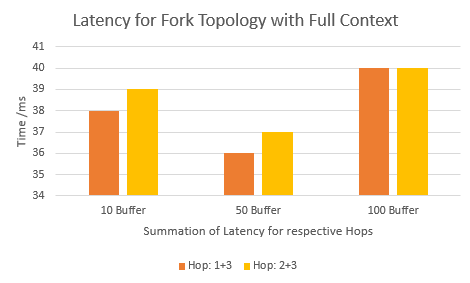
\includegraphics[width=\textwidth]{figures/buffer-fork.PNG}
	\caption{Latency for Fork Topology with Full Context}
	\label{fig:forktopo_latency_buffer_bar}
\end{figure}

\begin{figure}[H]
	\center
	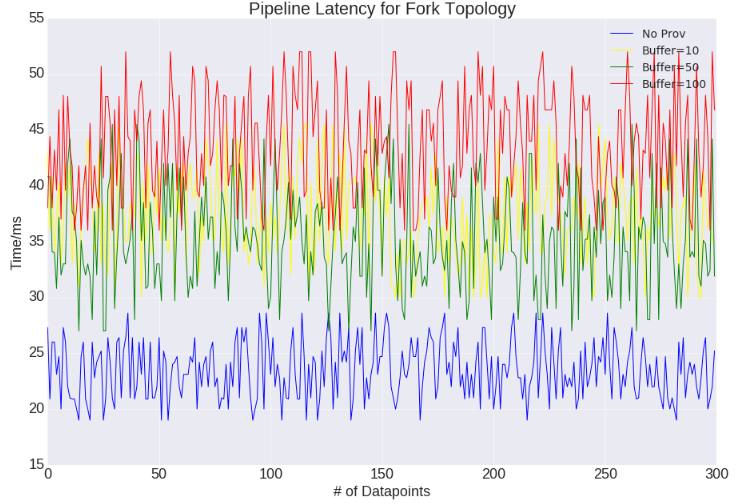
\includegraphics[width=\textwidth]{figures/pipeline_buffer.png}
	\caption{Pipeline Latency for Fork Topology with Full Context (Sum of Hop:1 and Hop:3 \ref{fig:fork_topo} using subsample of collected Data points)}
	\label{fig:forktopo_latency_buffer}
\end{figure}


\paragraph*{Conclusion}
As seen from figure \ref{fig:forktopo_latency_buffer} and figure\ref{fig:forktopo_latency_buffer} that the provenance system perform better when the buffer capacity setting is set to 50 messages. The reason behind this could be the implementation of the pipeline itself and also consider another functionality of the provenance system HeartBeat messages of the system which create network overhead. Latency difference could also be due to the bottleneck of the GatewayC. Fifty multiply by message size sent is a perfect size for the network bandwidth used by the service hence the difference in changing the buffer size explained without making a network congestion on the whole system being the sweet spot of the provenance system.


